\chapter{Organizzazioni e Soggetti coinvolti}
\label{chap:soggetti}

\section{Carbon Portal}
\label{section:carbonportal}
Il Carbon Portal è il portale web ufficiale di ICOS 
per l'accesso e la condivisione dei dati e delle
informazioni relative al monitoraggio
del ciclo del carbonio e dei gas serra in Europa.\\

Il Carbon Portal di ICOS offre una vasta gamma di servizi e
strumenti per la visualizzazione e l'analisi dei dati,
tra cui mappe interattive, grafici, tabelle e altri strumenti
di visualizzazione dei dati.
Inoltre, il portale fornisce un accesso unico a tutti i
dati e prodotti ICOS,
nonché a informazioni dettagliate sulle attività di
monitoraggio e sui protocolli di misura utilizzati.\\

Il servizio fornito dal Carbon Portal è hostato dall'Università di Lund
(in Svezia) \cite{LundUniversityICOS}
e dall'Università di Wageningen (in Olanda) \cite{WageningenUniversityICOS}.
Tutti i dati disponibili sono a cura dei Thematic Centres e del CAL.
Il Carbon Portal deve inoltre assicurare tutti gli aspetti legati
che circondano la qualità a 360° del dato tra cui la 
sicurezza di questi, fare in modo che i dati siano user-friendly e
soprattutto machine-friendly. Inoltre, la potenza del
Carbon Portal si può ritrovare nell'essere un univo
punto di accesso integrativo
per tutti gli utenti e le parti interessate ICOS,
che vanno da esperti al grande pubblico e supporta
protocolli e tecniche avanzate di scambio di dati, ampiamente standardizzate.
In particolare, tra le attività e le caratteristiche di tale servizio troviamo:
\begin{itemize}
    \item \textbf{Archiviazione a lungo termine e servizio di backup}.
    Il Carbon Portal deve organizzare l'archiviazione 
    a lungo termine dei dati ICOS
    prodotti, con l'obiettivo di garantirne la sicura
    archiviazione e gli accessi futuri (anche dopo un possibile
    cessazione dell'infrastruttura di ricerca stessa).
    \item \textbf{Data mining e data extraction}.
    Le funzionalità di ricerca consentono agli utenti di
    individuare e recuperare i dati di interesse, ad esempio,
    limitando la ricerca a specifici tipi di variabili,
    aree geografiche o periodi di tempo.
    \item \textbf{Mantenere gli standard sui dati e metadati}.
    L'armonizzazione degli standard di dati e metadati, è 
    responsabilità del Carbon Portal. Gli standard sui metadati,
    (come ad esempio, ISO 19115, Dublin Core, DIF) così come
    l'applicazione dello standard della direttiva INSPIRE
    (Infrastructure for Spatial Information in the European
    Community,vdirettiva dell'Unione Europea che mira
    a creare un'infrastruttura di scambio di informazioni
    geografiche interoperabile a livello europeo).
    \item \textbf{Fornire un servizio web pubblico}.
    Per agevolare molteplici operazioni sui dati, il Carbon
    Portal mette a disposizione un servizio web pubblico, come si
    può notare dalla figura seguente \ref{figure:carbonportalweb}

    \begin{figure}[h!]
        \centering
        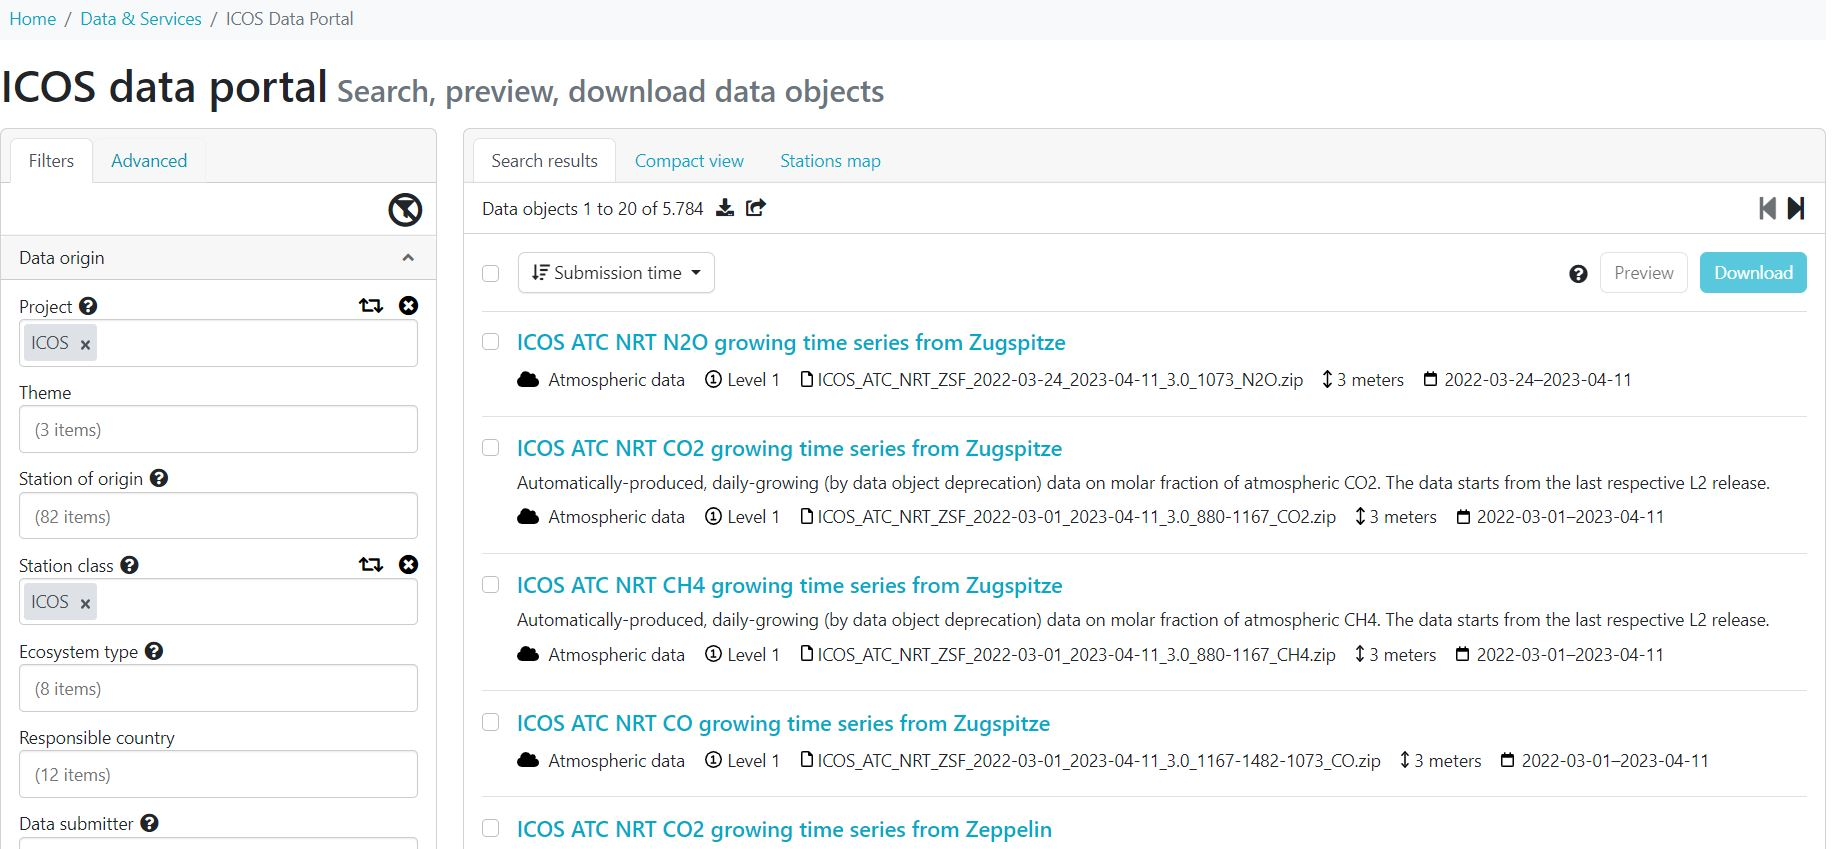
\includegraphics[height=0.5\textwidth]{figures/carbonportalweb.JPG}
        \caption{Interfaccia web messa a disposizione dal Carbon Portal.}
        \label{figure:carbonportalweb}
    \end{figure}

    L'interfaccia web fornisce un impressionante numero di informazioni
    e permette all'utente di analizzare i dati in maniera immediata e
    intuitiva grazie anche alla possibilità di creare istantaneamente
    dei grafici sui dati di nostro interesse. La figura \ref{figure:scatterchart} 
    mostra un esempio
    con un grafico a dispersione.

    \begin{figure}[h!]
        \centering
        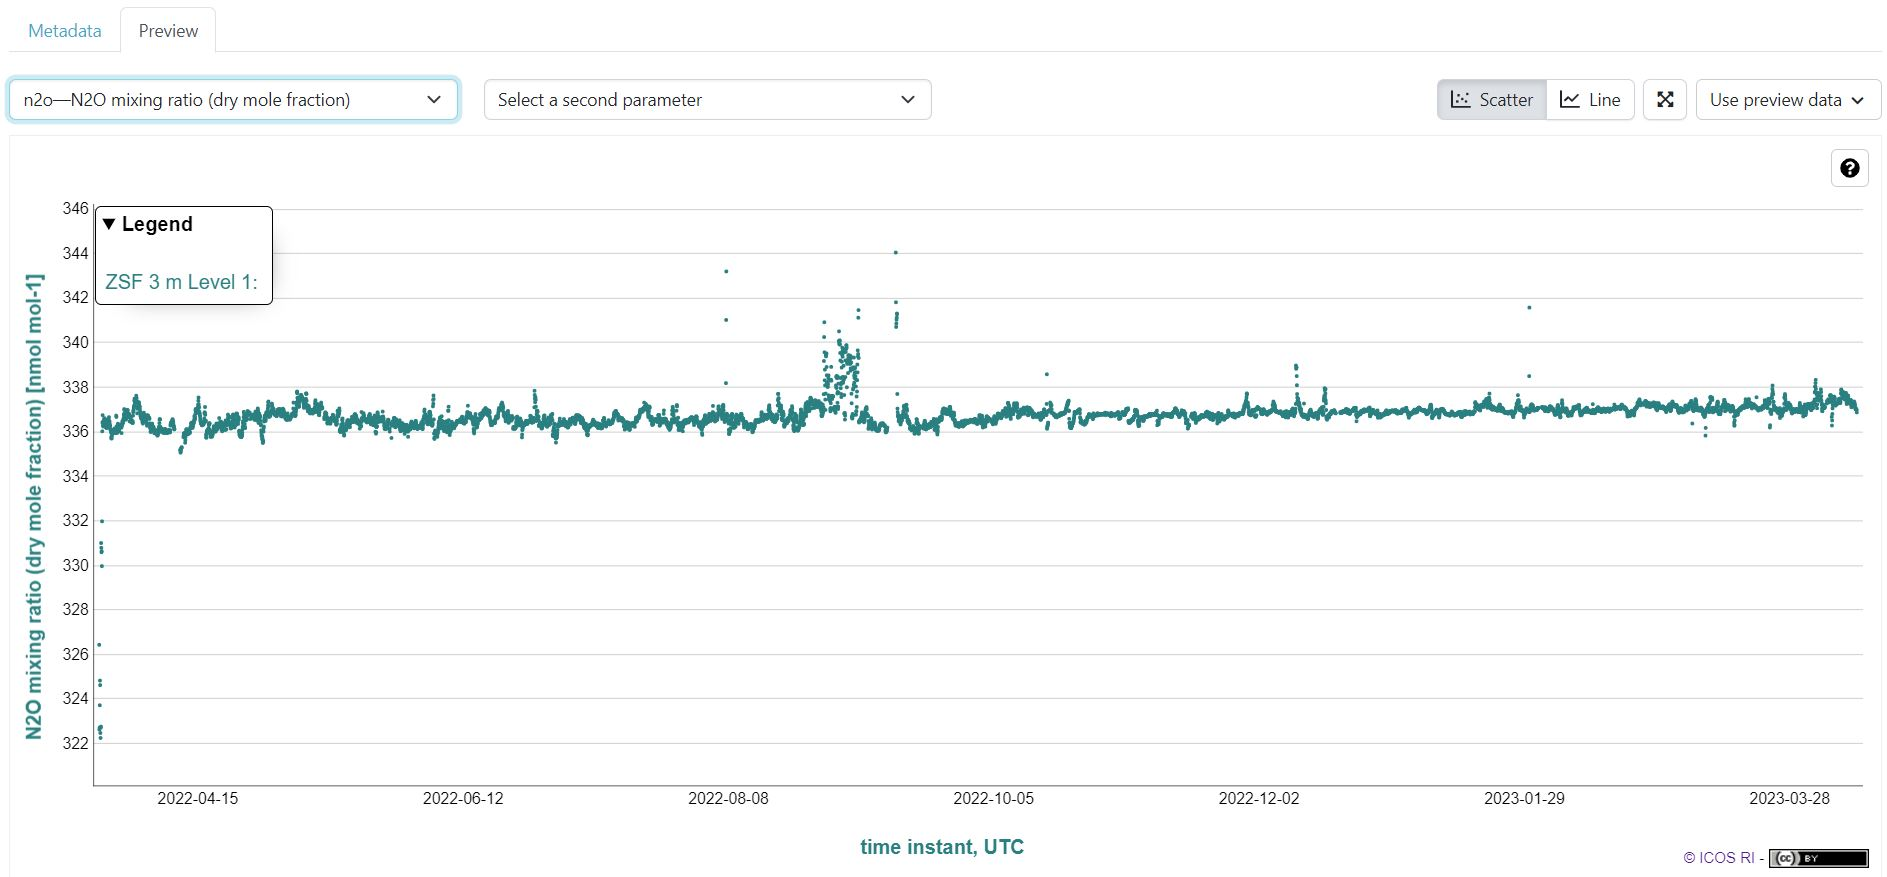
\includegraphics[height=0.5\textwidth]{figures/icosscatterchart.JPG}
        \caption{Esempio di una grafico a dispersione su dati d'esempio. Si noti la possibilità
        di scegliere il tipo di grafico e tante altre personalizzazioni.}
        \label{figure:scatterchart}
    \end{figure}


    \item \textbf{Interfacciarsi con i più importanti data portals europei e non}.
    Esiste un accordo, con altri centri di ricerca e
    data centers,
    su un formato univoco per
    lo scambio dei metadati così da facilitarne lo stesso.
    Carbon Portal collabora inoltre con queste realtà
    per garantire l'accessibilità reciproca a questi dati.
\end{itemize}

\section{Thematic Centres}
\label{section:thematic}
ICOS ricava informazioni da tre diverse tipologie di ambiente:
osservazioni atmosferiche, ecosistemiche e oceaniche. Ogni
tipologia di dato, viene raccolto dal relativo centro di osservazioni,
specializzato in analisi e manutenzione delle infrastrutture sul proprio
specifico dato.

\begin{itemize}
    \item \textbf{Atmosphere Thematic Centre}.\\
    ICOS ha istituito una rete di torri e stazioni
    (localizzate sia in alture di montagna sia in vicinanza
    di centri urbani)
    dove vengono raccolti i dati sulle concentrazioni di gas
    serra 
    nell'atmosfera \cite{AtmosphereObservationsICOS}. Le stazioniche si trovano lontano dai
    principali agenti inquinanti atmosferici, ad esempio
    nell'Artico o nelle Alpi, meglio
    rappresentano i cambiamenti nella composizione
    dei gas serra, rispetto ai siti più inquinati.
    A causa della loro elevazione e della distanza dalle
    principali fonti di gas serra,
    le stazioni remote sono principalmente esposte
    alle masse d'aria che rappresenteranno le
    condizioni atmosferiche sull'Europa centrale.
    Al contrario, le stazioni situate all'interno o
    in prossimità delle città sono importanti per
    comprendere le emissioni urbane; queste stazioni
    svolgono un ruolo cruciale nell'affrontare
    l'inquinamento urbano e aiutano a verificare
    i limiti internazionali di gas serra.\\

    L'ATC \cite{ICOSAtmosphereThematicCentre} è composto da tre unità: il \textit{Metrology Lab}, il quale
    esegue regolarmente controlli e analisi sulle tecnologie di misurazione,
    il \textit{Data Centre}, che sviluppa e mantiene il software
    per l'elaborazione dei dati ed esegue i controlli di qualità su di essi,
    ed infine il \textit{Mobile Lab}, il quale esegue misurazioni e controlli
    paralleli alle stazioni di monitoraggio direttamente sul campo.

    \item \textbf{Ocean Thematic Centre}.\\
    L'oceano è un fattore di vitale importanza nel ciclo di assorbimento
    di CO2 (assorbe circa il 25\% di anidride carbonica prodotta), è quindi
    necessario monitorare questo macro-sistema in relazione ai gas serra.
    La rete di stazioni oceaniche ICOS monitorano i gas serra
    nell'Atlantico e nei mari nordici, baltici e mediterranei \cite{OceanObservationsICOS}.
    I dati raccolti presso le stazioni oceaniche vengono elaborati
    e sottoposti a controllo qualitativo dall'Ocean Thematic Centre,
    che coordina la rete delle stazioni oceaniche.\\

    L'OTC coordina 22 stazioni oceaniche in 7 paesi, monitorando
    l'assorbimento e i flussi di carbonio nell'Atlantico settentrionale
    e nei mari nordici, baltici e mediterranei \cite{ICOSOceanThematicCentre}.
    I metodi di misurazione non solo prevedono la rilevazione da strutture
    fisse ma
    soprattutto da navi da ricerca,
    ormeggi, boe e navi commerciali. Questa unità di rilevazione
    marittima è strutturata in 5 divisioni: 
    \textit{Executive Unit} (coordina l'OTC),
    \textit{Labelling Unit} (coordina le attività di
    labelling dei dati),
    \textit{Data Unit} (a capo della raccolta dati
    e verifica della qualità),
    \textit{Training Unit} (servizio tecnico legato
    alla calibrazione delle strumentazioni e del corretto
    impiego di esse) ed infine il
    \textit{New Technology and Platforms Unit} (si
    occupa di adottare nuovi sensori e strumentazioni,
    per rimanere sempre all'avanguardia).

    \item \textbf{Ecosystem Thematic Centre}.\\
    La rete di misurazione ICOS legata agli ecosistemi,
    misura i gas serra, nonché i componenti viventi
    e non viventi (ovvero i responsabili dello
    scambio di gas serra), acqua ed energia
    tra gli ecosistemi e l'atmosfera \cite{OceanObservationsICOS}. ICOS osserva
    i gas serra in vari tipi di ecosistemi.
    È importante capire in che modo i diversi
    ecosistemi rispondono ai cambiamenti climatici,
    ad esempio se sono o diventeranno pozzi, ovvero ambienti
    che aiuteranno a rimuovere i gas serra, o fonti
    di gas serra, che tenderanno a rilasciare CO2 o altri gas serra.\\

    Le raccolta dati dei gas serra negli ecosistemi terrestri
    è coordinata dall'ETC, l'Ecosystem Thematic Centre \cite{ICOSEcosystemThematicCentre}.
    L'ETC supporta le stazioni di monitoraggio piazzate nelle regioni
    di interesse, esegue l'elaborazione centralizzata
    dei dati e il controllo qualità su di essi e fornisce inoltre
    assistenza tecnica alle stazioni.
    L'ETC ha un ruolo fondamentale nello scambio di
    informazioni ambientali
    con la comunità scientifica, che gli ha permesso negli anni di
    sviluppare e testare nuovi metodi di
    elaborazione dei dati,
    tecniche di misurazione e strumenti utili al loro scopo. In particolare,
    l'ETC è composto da 5 sezioni: coloro che si occupano delle relazioni
    e del coordinamento dell'intero struttura (\textit{Executive Committee Unit}),
    chi si occupa del processo di collezione, archiviazione e controllo di
    qualità del dato (\textit{Data Unit}), il gruppo incaricato
    di valutare nuovi approcci alle misurazioni (\textit{Test Unit})
    ed infine la sezione responsabile dell'assistenza diretta alle
    stazioni (\textit{Network Unit}).
   


\end{itemize}

\section{ICOS Central Analytical Laboratories (CAL)}
\label{section:CAL}
Il CAL, Central Analytical Laboratories, è una delle strutture
principali di ICOS e lavora a supporto delle attività di monitoraggio \cite{ICOSCentralAnalyticalLaboratories}.
Il focus principale delle loro mansioni, è garantire l'accuratezza
dei dati di misurazione atmosferica. Questo prevede le seguenti attività:
\begin{itemize}
    \item Analisi dei parametri accessori nei campioni.
    di aria prelevati presso le stazioni di monitoraggio.
    \item Manutenzione e sviluppo delle attrezzature per il campionamento.
    \item Supporto delle attività di controllo qualità.
\end{itemize}